\documentclass[../main.tex]{subfiles}
\begin{document}
\graphicspath{{../imagenes/}}
\section{Filtros}

	% ------ SACCHI OCTAVIO ------ %
	\subsection{Introduccion}	
	Un filtro es un circuito que, dependiendo de su configuración, atenúa, rechaza o corrige
	un cierto rango de frecuencia de una señal.

	Hay dos tipos principales de filtros: Filtros activos y Filtros pasivos, estos
	se califican por los componentes que utlizan.\\
	Sus características principales son la siguientes:
	\begin{itemize}
		\item Filtros Pasivos:\\ Los filtros pasivos son los filtros cuyos componentes no
			requieren una alimentacion externa para funcionar, sino que solo requieren una 
			señal de entrada
		\item Filtros Activos:\\ Los filtros activos son los filtros cuyos componentes si
			requieren una alimentacion externa para funcionar
	\end{itemize}

	Existen varios subtipos de filtros, entre los que destacan estan los filtros 
	pasa bajos, pasa altos, pasa banda y rechaza banda \\ 


	\subsection{Pasivos}
	Los filtros pasivos usan componentes básicos tales como 
	una resistencia, un capacitor o una bobina, son fáciles de
	hacer, pero los filtros pasivos son difíciles de ajustar
	y tienen una baja potencia, además son incapaces de 
	eliminar el rango de frecuencia no deseado.
	
	Poseen algunas variaciones que son los de un solo elemento,
	de múltiples elementos, variaciones de T, pi y L.
	\begin{figure}[H]
		\includegraphics[width=0.6 \textwidth]{filtros/filtro_pasivo.png}
		\centering
		\caption{Circuito de un filtro pasivo}
	\end{figure}


{	
	\renewcommand{\subsectionbreak}{}
	\subsection{Activos}
	Los filtros activos utilizan componentes básicos de los 
	filtros pasivos, pero se les agrega componentes más complicados
	como un amplificador operacional, provocando que el filtro sea
	más fácil de ajustar, pueden amplificar la señal, pueden obtene
	r una mayor potencia y son capaces de eliminar rangos de 
	frecuencia no deseados.
	\begin{figure}[H]
		\includegraphics[width=0.6 \textwidth]{filtros/filtro_activo.png}
		\centering
		\caption{Circuito de un filtro activo}
	\end{figure}
}


	% ------- KRAPP RAMIRO ------- %
	%--------------------------------------------%
	%---------------- PASA BAJOS ----------------%
	%--------------------------------------------%
	\subsection{Pasa Bajos}
	Un filtro pasa bajos es un filtro de señales electrónicas, que bloquea señales de alta
	frecuencia.

	Este tambien puede ser visto como si ``dejara pasar'' señales de baja frecuencia, de aqui
	la razón del nombre.

	Hay dos formas de hacer un filtro pasa bajos:

	%---------------- PASA BAJOS CON CAPACITORES ----------------%

		\subsubsection{Filtro usando capacitores}
		Una forma de hacer un filtro pasa bajos es usando un capacitor conectado 
		de la siguiente forma:
		\begin{figure}[H]
			\centering
			\includegraphics[width=0.5\textwidth]{filtros/pasa-bajo_cap1.pdf}
			\caption{Un filtro pasa bajos capacitivo}
		\end{figure}
		Su funcionamiento se puede deducir viendo la fórmula de impedancia del capacitor:
		\[
			X_C = \dfrac{-J}{2\pi \x f \x C}
		\]
		\begin{wrapfigure}{r}{0in}
			\centering
			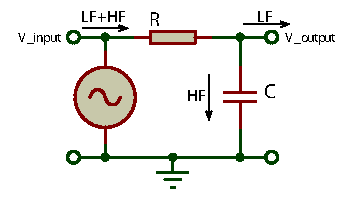
\includegraphics[width=0.4\textwidth]{filtros/pasa-bajo_cap2.pdf}
			\caption{\centering{Un diagrama  que ejemplifica el funcionamiento}}
		\end{wrapfigure}
		Como se ve en la formula, con una frecuencia ($f$) baja se obtiene una gran 
		inductancia, y a medida que aumentamos la frecuencia ($f$) la inductancia va 
		disminuyendo. \\\\
		Esto logra que todas las señales entren al filtro, pero que las señales de alta
		frecuencia se vean atraidas a circular por el capacitor debido a su baja inductancia
		ante las señales de alta frecuencia, por lo tanto a la salida del filtro logramos
		tener solamente señales de baja frecuencia. \\\\
		Para saber con que frecuencias operará el filtro, se debe conocer la
		\emph{frecuencia de corte}.\\
		El filtro bloqueara todas las frecuencias que esten por arriba
		de esta frecuencia.\\
		Esta frecuencia de corte se calcula con la siguiente formula:
		\[
			f_{cut} = \dfrac{1}{2\pi \x R \x C}
		\]
		Esta equivale a 3dB o 0.707V\\
		Cuando $f = f_{cut}$ se da que $R = \left | XC \right |$

	 %---------------- PASA BAJOS CON INDUCTORES ----------------%
	
		\clearpage
		\subsubsection{Filtro usando inductores}
		Una forma de hacer un filtro pasa bajos es usando un inductor conectado 
		de la siguiente forma:
		\begin{figure}[H]
			\centering
			\includegraphics[width=0.5\textwidth]{filtros/pasa-bajo_ind1.pdf}
			\caption{Un filtro pasa bajos inductivo}
		\end{figure}
		Su funcionamiento se puede deducir viendo la fórmula de impedancia del inductor:
		\[
			X_L =J \x 2\pi \x f \x L
		\]
		\begin{wrapfigure}{r}{0in}
			\centering
			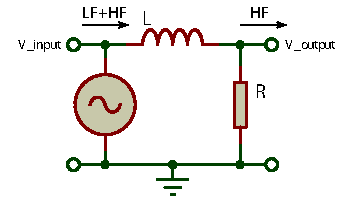
\includegraphics[width=0.4\textwidth]{filtros/pasa-bajo_ind2.pdf}
			\caption{\centering{Un diagrama que ejemplifica el funcionamiento}}
		\end{wrapfigure}
		Como se ve en la fórmula, con una frecuencia ($f$) baja se obtiene una baja 
		inductancia, y a medida que aumentamos la frencuencia ($f$) la inductancia 
		va aumentando.\\\\
		Esto logra que las señales de alta frecuencia se encuentren con una alta inductancia
		en la entrada, mientras que las señales de baja frecuencia se encuentran con 
		una baja inductancia en la entrada, por lo tanto solamente estas últimas logran
		atravezar el filtro.\\\\
		Para saber con que frecuencias operará el filtro, se debe conocer la
		\emph{frecuencia de corte}.\\
		El filtro bloqueara todas las frecuencias que esten por arriba
		de esta frecuencia.\\
		Esta frecuencia de corte se calcula con la siguiente formula:
		\[
			f_{cut} = \dfrac{R}{2\pi \x L}
		\]
		Esta equivale a 3dB o 0.707V\\
		Cuando $f = f_{cut}$ se da que $R = \left | XL \right |$

		\begin{figure}[H]
			\centering
			\includegraphics[width=0.7\textwidth]{filtros/pasa-bajo_grafico.png}
			\caption{Un gráfico simplificado de la respuesta en frecuencia}
		\end{figure}
	%--------------------------------------------%
	%---------------- PASA ALTOS ----------------%
	%--------------------------------------------%
	\subsection{Pasa Altos}
	Un filtro pasa altos es un filtro de señales electrónicas, que bloquea señales de baja
	frecuencia. \\
	Este tambien puede ser visto como si ``dejara pasar'' señales de alta frecuencia, de aqui
	la razón del nombre. \\
	Hay dos formas de hacer un filtro pasa altos:

	%---------------- PASA ALTOS USANDO CAPACITORES ----------------%

		\subsubsection{Filtro usando capacitores}
		Una forma de hacer un filtro pasa altos es usando un capacitor conectado 
		de la siguiente forma:
		\begin{figure}[H]
			\centering
			\includegraphics[width=0.5\textwidth]{filtros/pasa-alto_cap1.pdf}
			\caption{Un filtro pasa altos capacitivo}
		\end{figure}
		Su funcionamiento se puede deducir viendo la fórmula de impedancia del capacitor:
		\[
			X_C = \dfrac{-J}{2\pi \x f \x C}
		\]
		\begin{wrapfigure}{r}{0in}
			\centering
			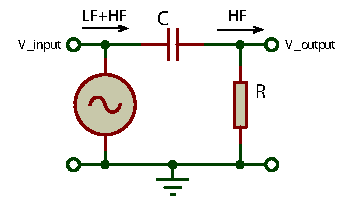
\includegraphics[width=0.4\textwidth]{filtros/pasa-alto_cap2.pdf}
			\caption{\centering{Un diagrama que ejemplifica el funcionamiento}}
		\end{wrapfigure}
		Como se ve en la formula, con una frecuencia ($f$) baja se obtiene una gran 
		inductancia, y a medida que aumentamos la frecuencia ($f$) la inductancia va 
		disminuyendo. \\\\
		Esto logra que las señales de baja frecuencia se encuentren con una gran inductancia
		en la entrada, mientras que las señales de alta frecuencia se encuentran con 
		una baja inductancia en la entrada, por lo tanto solamente estas últimas logran
		atravezar el filtro. \\\\
		Para saber con que frecuencias operará el filtro, se debe conocer la
		\emph{frecuencia de corte}.\\
		El filtro bloqueara todas las frecuencias que esten por debajo
		de esta frecuencia.\\
		Esta frecuencia de corte se calcula con la siguiente formula
		\[
			f_{cut} = \dfrac{1}{2\pi \x R \x C}
		\]
		Esta equivale a 3dB o 0.707V\\
		Cuando $f = f_{cut}$ se da que $R = \left| XC \right|$


	%---------------- PASA ALTOS USANDO INDUCTORES ----------------%
		\clearpage
		\subsubsection{Filtro usando inductores}
		Una forma de hacer un filtro pasa altos es usando un inductor conectado 
		de la siguiente forma:
		\begin{figure}[H]
			\centering
			\includegraphics[width=0.5\textwidth]{filtros/pasa-alto_ind1.pdf}
			\caption{Un filtro pasa altos inductivo}

		\end{figure}
		Su funcionamiento se puede deducir viendo la fórmula de impedancia del inductor:
		\[
			X_L =J \x 2\pi \x f \x L
		\]
		\begin{wrapfigure}{r}{0in}
			\centering
			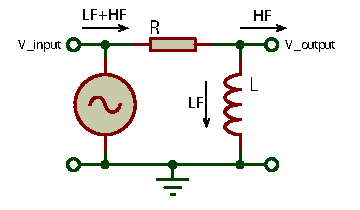
\includegraphics[width=0.4\textwidth]{filtros/pasa-alto_ind2.pdf}
			\caption{\centering{Un diagrama que ejemplifica el funcionamiento}}
		\end{wrapfigure}
		Como se ve en la fórmula, con una frecuencia ($f$) baja se obtiene una baja 
		inductancia, y a medida que aumentamos la frencuencia ($f$) la inductancia 
		va aumentando. \\\\
		Esto logra que todas las señales entren al filtro, pero que las señales de baja
		frecuencia se vean atraidas a circular por el indudctor debido a su baja inductancia
		ante las señales de baja frecuencia, por lo tanto a la salida del filtro logramos
		tener solamente señales de alta frecuencia. \\\\
		Para saber con que frecuencias operará el filtro, se debe conocer la
		\emph{frecuencia de corte}.\\
		El filtro bloqueara todas las frecuencias que esten por debajo 
		de esta frecuencia. \\
		Esta frecuencia de corte se calcula con la siguiente formula:
		\[
			f_{cut} = \dfrac{R}{2\pi \x L}
		\]
		Esta equivale a 3dB o 0.707V\\
		Cuando $f = f_{cut}$ se da que $R = \left | XL \right |$

		\begin{figure}[H]
			\centering
			\includegraphics[width=0.7\textwidth]{filtros/pasa-alto_grafico.png}
			\caption{Un gráfico simplificado de la respuesta en frecuencia}
		\end{figure}

	\subsection{Impedancia en respuesta a la frecuencia}
	\begin{figure}[H]
		\centering
		\includegraphics[width= 0.9\textwidth]{filtros/impedancia_capacitiva.png}
		\caption{Grafico de la impedancia de un capacitor en respuesta de la frecuencia}
	\end{figure}\begin{figure}[H]
		\centering
		\includegraphics[width=0.9\textwidth]{filtros/impedancia_inductiva.png}
		\caption{Grafico de la impedancia de un inductor en respuesta de la frecuencia}
	\end{figure}


	%--------------------------------------------%
	%---------------- PASA BANDA ----------------%
	%--------------------------------------------%
	\subsection{Pasa Banda}
	Un filtro pasa banda es un filtro de señales electrónicas, que bloquea tanto señales 
	de baja frecuencia como señales de alta frecuencia. \\
	Este tambien puede ser visto como si ``dejara pasar'' una cierta banda de frecuencias,
	de aqui la razón del nombre. \\
	Un filtro pasa banda se puede elaborar de la siguiente forma
	\begin{figure}[H]
		\centering
		\includegraphics[width=0.5\textwidth]{filtros/pasa-banda_cap1.pdf}
		\caption{Un filtro pasa banda capacitivo}
	\end{figure}

	Este filtro es una combinación entre un filtro pasa altos y un filtro pasa bajos,
	su efecto se puede ver en la figura \ref{pasa-banda_grafico}.
	\begin{figure}[H]
		\centering
		\includegraphics[width=0.7\textwidth]{filtros/pasa-banda_grafico.png}
		\caption{Un gráfico simplificado de la respuesta en frecuencia}
		\label{pasa-banda_grafico}
	\end{figure}



	\subsection{Rechaza Banda}
	Un filtro rechaza-banda es el contrario a un filtro pasa banda, siendo que atenua todas las frecuencias en un dentro de un determinado ancho de banda y deja pasar las que están por fuera de este ancho de banda.
	\begin{figure}[H]
		\centering
		\includegraphics[width=0.7\textwidth]{filtros/rechaza-banda_grafico1.png}
	\end{figure}

	Existen dos tipos de filtros rechaza-banda, el anterior grafico corresponde al
	tipo de banda amplia, aunque también existen los de banda angosta:
	\begin{figure}[H]
		\centering
		\includegraphics[width=0.7\textwidth]{filtros/rechaza-banda_grafico2.png}
	\end{figure}
	
	\begin{wrapfigure}{r}{0in}
		\includegraphics[width=0.3\textwidth]{filtros/rechaza-banda_circuito1.png}
	\end{wrapfigure}
	Para obtener este filtro hay dos maneras de crearlo, usando un circuito de resonancia serie o uno paralelo, cuando la frecuencia de Vi sea igual a la de resonancia.
	En el circuito LC tiene baja impedancia.

	El armado es similar a un filtro pasa banda pero la diferencia está en la 
	ubicación de las salidas del filtro, pues en el pasa banda la salida del
	filtro se encontraba en la resistencia, por lo que a F resonancia veíamos 
	en la salida toda la tensión de entrada, pero ahora en 
	la salida tenemos el LC por lo que no habrá caída de tensión.\\

	En el caso contrario, que la frecuencia sea distinta a la de resonancia,
	el conjunto LC actuara con una impedancia muy alta, por lo que la tensión
	caerá en este y habrá salida de tensión en el filtro.

	Con este análisis podemos llegar a ver que hay un divisor de tensión entre
	la impedancia del circuito LC y la resistencia.\\

	El análisis del circuito paralelo es similar, únicamente que funciona a 
	máxima impedancia en la frecuencia de resonancia y a mínima
	impedancia lejos de las frecuencias de resonancia, y como ya dijimos esto
	funciona como un divisor de tensión y como tenemos la salida en la 
	resistencia al llegar a la frecuencia de resonancia habrá máxima impedancia y se provocará
	un divisor de tensión en donde toda la tensión caerá en el circuito de resonancia LC
	dejando sin tensión a la salida, y por el caso contrario, cuando al frecuencia se aleja
	de la F resonancia la impedancia disminuye lo que provoca que haya una caída de tensión
	en la R por lo que hay salida de tensión. 

	Otra forma de ver el armado podría ser poniendo un amplificador sumador a un filtro
	pasa bajos y uno pasa bajos, donde usamos el pasa bajos para poder encontrar la
	frecuencia de corte 1 y el pasa alto para encontrar la frecuencia de corte 2

	\begin{figure}[H]
		\centering
		\includegraphics[width=\textwidth]{filtros/rechaza-banda_circuito2.png}
	\end{figure}

	Para poder calcular la frecuencia de corte 1 empezamos calculando el filtro
	pasa bajos, supongamos que queremos crear un filtro rechaza-banda de
	10Hz a 100Hz, primero empezamos calculando un pasa bajos con frecuencia 
	de corte 10Hz, usando la formula
	\[
		F_{corte} = \dfrac {1}{2\pi \x R1 \x C1}
	\]
	Luego calculamos la frecuencia de corte del filtro pasa altos
	con la misma fórmula pero en la F de corte cambiamos, en este caso, 10Hz a 100Hz.

\end{document}
